\documentclass[12pt,a4paper]{report}

\usepackage[utf8]{inputenc}
\usepackage[T1]{fontenc}
\usepackage{lmodern}
\usepackage{geometry}
\usepackage{setspace}
\usepackage{titlesec}
\usepackage{titletoc}
\usepackage{tocloft}
\usepackage{fancyhdr}
\usepackage{graphicx}
\usepackage{xcolor}
\usepackage{booktabs}
\usepackage{longtable}
\usepackage{array}
\usepackage{multirow}
\usepackage{tabularx}
\usepackage{enumitem}
\usepackage{caption}
\usepackage{subcaption}
\usepackage{float}
\usepackage{hyperref}
\usepackage{url}
\usepackage{listings}
\usepackage{tikz}
\usepackage{amsmath}
\usepackage{amssymb}
\usepackage{csquotes}
\usepackage{appendix}
\usepackage[numbers,sort&compress]{natbib}

\usetikzlibrary{arrows.meta,positioning,shapes.geometric,fit,calc}

\geometry{
  left=3.0cm,
  right=2.5cm,
  top=2.5cm,
  bottom=2.5cm
}

\onehalfspacing
\setlength{\parindent}{1.0cm}
\setlength{\parskip}{0pt}
\setlist[itemize]{topsep=3pt,itemsep=2pt,parsep=0pt}
\setlist[enumerate]{topsep=3pt,itemsep=2pt,parsep=0pt}

\definecolor{usthblue}{HTML}{1F4E79}
\definecolor{softblue}{HTML}{EAF2F8}
\definecolor{softgray}{HTML}{F4F6F8}
\definecolor{codegray}{HTML}{F7F7F7}
\definecolor{codeborder}{HTML}{D9E2EC}

% Re-format chapter and section titles to match template
\titleformat{\chapter}[display]
  {\normalfont\bfseries\color{usthblue}}
  {\chaptertitlename\ \thechapter}{12pt}{\LARGE}
\titleformat{\section}
  {\normalfont\Large\bfseries\color{usthblue}}
  {\thesection}{0.8em}{}
\titleformat{\subsection}
  {\normalfont\large\bfseries\color{usthblue}}
  {\thesubsection}{0.8em}{}
\titleformat{\subsubsection}
  {\normalfont\normalsize\bfseries}
  {\thesubsubsection}{0.8em}{}

\captionsetup{font=small,labelfont=bf}
\renewcommand{\cftchapfont}{\bfseries}
\renewcommand{\cftchappagefont}{\bfseries}

% Setup running headers and footers matching the ADAS template format
\pagestyle{fancy}
\fancyhf{}
\fancyhead[R]{Camera AI USTH 2026}
\fancyfoot[C]{\thepage}
\renewcommand{\headrulewidth}{0.4pt}

% Redefine the plain page style (used on chapter start pages) so headers are retained
\fancypagestyle{plain}{
  \fancyhf{}
  \fancyhead[R]{Camera AI USTH 2026}
  \fancyfoot[C]{\thepage}
  \renewcommand{\headrulewidth}{0.4pt}
}

\lstdefinestyle{pythonstyle}{
  backgroundcolor=\color{codegray},
  frame=single,
  rulecolor=\color{codeborder},
  basicstyle=\ttfamily\small,
  breaklines=true,
  columns=fullflexible,
  keepspaces=true,
  showstringspaces=false,
  keywordstyle=\color{usthblue}\bfseries,
  commentstyle=\color{gray},
  stringstyle=\color{teal}
}

\newcommand{\projecttitle}{Camera AI Attendance System Using Real-Time Face Recognition}
\newcommand{\studentname}{Dang Binh An}
\newcommand{\studentid}{23BI14005}
\newcommand{\internalsupervisor}{Tran Hoang Tung}
\newcommand{\externalsupervisor}{Pham Van Dan}
\newcommand{\academicyear}{2025--2026}

\begin{document}

% --- Cover Page (No page number, no header) ---
\begin{titlepage}
  % Khung viền kép (Double border) giống hình mẫu
  \begin{tikzpicture}[remember picture, overlay]
    % Viền ngoài (đậm)
    \draw[line width=1.5pt] 
      ($(current page.north west) + (2.0cm, -2.0cm)$) 
      rectangle 
      ($(current page.south east) + (-1.5cm, 2.0cm)$);
    % Viền trong (mảnh)
    \draw[line width=0.5pt] 
      ($(current page.north west) + (2.1cm, -2.1cm)$) 
      rectangle 
      ($(current page.south east) + (-1.6cm, 2.1cm)$);
  \end{tikzpicture}

  \centering
  \vspace*{0.2cm}
  {\large\bfseries UNIVERSITY OF SCIENCE AND TECHNOLOGY\par}
  {\large\bfseries OF HANOI\par}
  \vspace{0.2cm}
  {\normalsize\bfseries VIETNAM FRANCE UNIVERSITY\par}
  
  \vspace{1.5cm}

  % USTH Logo
  \IfFileExists{usth_logo.png}{
    \includegraphics[width=6.5cm]{usth_logo.png}\par
  }{
    
\begin{tikzpicture}
      \draw[thick, dashed] (0,0) rectangle (6.5, 2.5);
      \node[align=center] at (3.25, 1.25) {\small\bfseries USTH LOGO\par\scriptsize (Place usth\_logo.png here)};
    \end{tikzpicture}\par
  }

  \vspace{1.5cm}

  % Hai đường gạch ngang bao quanh tên Thesis
  \rule{0.85\textwidth}{0.8pt} \par
  \vspace{0.5cm}
  {\Large\bfseries FINAL THESIS\par}
  \vspace{0.3cm}
  {\large\bfseries \projecttitle\par}
  \vspace{0.4cm}
  \rule{0.85\textwidth}{0.8pt} \par

  \vspace{2.0cm}

  % Thông tin Sinh viên & Giảng viên (Chỉ in đậm tiêu đề theo ảnh)
  {\large \textbf{Student:} \studentname\ - \studentid\par}
  \vspace{0.6cm}
  {\large \textbf{Internal Supervisor:} \internalsupervisor\par}
  \vspace{0.6cm}
  {\large \textbf{External Supervisor:} \externalsupervisor\par}

  \vfill

  % Thông tin Năm học & Địa điểm
  {\large\bfseries Academic Year: \academicyear\par}
  \vspace{0.3cm}
  {\large Hanoi, July 2026\par}
  \vspace{0.5cm}
\end{titlepage}

% --- Sequential Arabic Page Numbering starting from Certification Page ---
\pagenumbering{arabic}
\setcounter{page}{1}

% --- Supervisor Certification Page ---
\chapter*{Supervisor Certification}
\addcontentsline{toc}{chapter}{Supervisor Certification}
To whom it may concern,

I, \externalsupervisor, certify that the thesis/internship report of Mr. \studentname\ is qualified to be presented in the Internship Jury \academicyear.

\vspace{1.5cm}
\begin{flushright}
  \begin{minipage}{0.4\textwidth}
    \centering
    Hanoi, July 2026 \\[1.5cm]
    Supervisor's signature
  \end{minipage}
\end{flushright}

\clearpage

% --- Acknowledgements Page ---
\chapter*{Acknowledgements}
\addcontentsline{toc}{chapter}{Acknowledgements}
I would like to express my heartfelt gratitude to all those who supported me throughout the course of my internship and the completion of this thesis.

First and foremost, I wish to extend my deepest gratitude to my external supervisor, \externalsupervisor. More than a mentor, he has been a true companion throughout this journey. It has been a great honor to work with you, and I am incredibly grateful for the invaluable guidance, resources, and supportive working environment that I received during the development of this project.

I would also extend my sincere thanks to my internal supervisor, \internalsupervisor, for his insightful feedback, academic support, and continuous encouragement throughout this project.

To my dear family, thank you for the unwavering emotional support and encouragement, which kept me motivated and grounded during this journey. Whatever I do will never be enough to express my love for all of you.

And finally, to my friends and colleagues at Vinorsoft, thank you for your help, guidance, and for providing a wonderful, collaborative environment during my internship.

\clearpage

% --- List of Abbreviations ---
\chapter*{List of Abbreviations}
\addcontentsline{toc}{chapter}{List of Abbreviations}
\begin{longtable}{p{3.5cm}p{10.5cm}}
\toprule
\textbf{Abbreviation} & \textbf{Meaning} \\
\midrule
AI & Artificial Intelligence \\
API & Application Programming Interface \\
CNN & Convolutional Neural Network \\
CPU & Central Processing Unit \\
CV & Computer Vision \\
DB & Database \\
DL & Deep Learning \\
FAISS & Facebook AI Similarity Search \\
FER & Facial Expression Recognition \\
FPS & Frames Per Second \\
HSV & Hue, Saturation, Value \\
JSON & JavaScript Object Notation \\
MTCNN & Multi-task Cascaded Convolutional Networks \\
ONNX & Open Neural Network Exchange \\
ORM & Object Relational Mapping \\
REST & Representational State Transfer \\
ROI & Region of Interest \\
SQL & Structured Query Language \\
SSD & Single Shot Detector \\
YOLO & You Only Look Once \\
\bottomrule
\end{longtable}

\clearpage

% --- Table of Contents, Lists ---
\tableofcontents
\clearpage
\listoffigures
\clearpage
\listoftables
\clearpage

% --- Body Chapters (Chapter 1 to 7) ---
\chapter{Introduction}

\section{Abstract}
This thesis presents the design, implementation, and empirical evaluation of a real-time Camera AI Attendance System using deep learning-based face recognition. The primary objective is to address the operational and security weaknesses of traditional attendance methods, such as paper sheets, manual signatures, and proxy-prone magnetic cards. The proposed system combines a multi-model face detection layer (supporting YOLOv8-face, MTCNN, and Haar Cascade fallbacks), a face verification module (InceptionResnetV1), and a lightweight facial expression recognition model (Mini-Xception) for emotion-gated interactions. To secure the check-in process against presentation attacks, we implement a rule-based 2D anti-spoofing mechanism utilizing Laplacian texture variance, HSV skin-color filtering, and Canny margin bezel checks. Additionally, a motion-waving gesture check-out module based on temporal frame difference is introduced to automate check-out events and filter out passive background pedestrians. The vision pipeline is integrated with a high-performance, asynchronous FastAPI backend and a web dashboard displaying real-time events. Real-time testing on an Intel Core i5 CPU demonstrates that the system achieves high verification accuracy at an operating threshold of $\theta_{\text{verify}} = 0.65$ and runs at a practical rate of 15--20 FPS (maximizing at 25.2 FPS with ROI-based tracking), demonstrating the viability of low-cost edge AI deployments.

\noindent\textbf{Keywords:} face recognition, attendance automation, Mini-Xception, FastAPI, anti-spoofing, real-time pipeline.

\section{Context and Motivation}
Attendance logging is a routine yet critical administrative task in modern organizations, including offices, universities, factories, and research facilities. Historically, organizations have relied on manual methods, such as paper sheets, signature books, and Excel logs, which are slow, error-prone, and require significant administrative labor. To address these issues, card-based systems (e.g., RFID, magnetic stripe cards) and barcode-based ID cards were widely adopted. While these methods digitalize the logs, they fail to prevent the phenomenon of "buddy punching" or proxy attendance, where employees swap cards to check in for absent colleagues. This practice leads to financial losses, inaccurate productivity metrics, and security vulnerabilities.

Biometric technologies, such as fingerprint scanners and iris recognition, offer a more secure alternative. However, fingerprint sensors require direct physical contact (which accelerates wear and tear and poses sanitation issues), and iris scanners are expensive and require active user cooperation at close range. In this context, camera-based Computer Vision (CV) has emerged as an ideal, non-contact biometric solution. Standard surveillance or web cameras can capture rich visual information from a distance, allowing deep learning models to automatically verify identities without requiring physical interaction or specialized hardware.

The motivation of this project is to develop and evaluate a complete, end-to-end Camera AI Attendance System during an internship at Vinorsoft. The system is designed to run efficiently on standard CPU-based edge hardware. Rather than treating face recognition as an isolated classification task, this project integrates computer vision models into a complete software architecture. Detections and embeddings are combined with business rules, persistent SQLite databases, and a real-time Web dashboard. This engineering approach bridges the gap between academic AI models and real-world software applications, providing an automated, contact-free check-in and check-out system.

\section{Project Objective}
The primary objective of this project is to build a functional, real-time camera-based attendance prototype that is reliable, secure, and easy to manage. To achieve this, the system incorporates the following objectives:
\begin{enumerate}
    \item \textbf{Robust Face Verification:} Implement a highly accurate face detection and recognition pipeline using open-source deep learning architectures (YOLOv8-face and InceptionResnetV1) capable of matching employees against a registered database using cosine similarity.
    \item \textbf{Liveness Detection:} Design a lightweight, real-time 2D anti-spoofing filter that detects screen replay or paper print attacks without introducing high computational latency.
    \item \textbf{Behavioral Interaction Gates:} Implement emotion-gated check-in (requiring a smiling face to register attendance) and hand-waving gesture check-out to verify active employee presence and distinguish checking-out individuals from passive passers-by.
    \item \textbf{Production-Grade Software Integration:} Wrap the vision pipeline in a FastAPI web service, using asynchronous WebSockets for live video annotation and logging, and construct a web dashboard for administrative CRUD operations and reports.
\end{enumerate}

\section{Desired Outcomes}
The project aims to achieve the following tangible outcomes:
\begin{itemize}
    \item A fully integrated software prototype containing the camera capture, backend server, database, and frontend dashboard.
    \item An operational real-time processing rate of at least 15 frames per second (FPS) on standard dual-core CPU machines.
    \item A robust verification accuracy with a low False Acceptance Rate (FAR) under controlled indoor lighting conditions.
    \item A reliable attendance state engine that correctly logs check-in (smile), check-out (wave), late arrivals, and cooldown periods.
\end{itemize}

\begin{figure}[H]
\centering
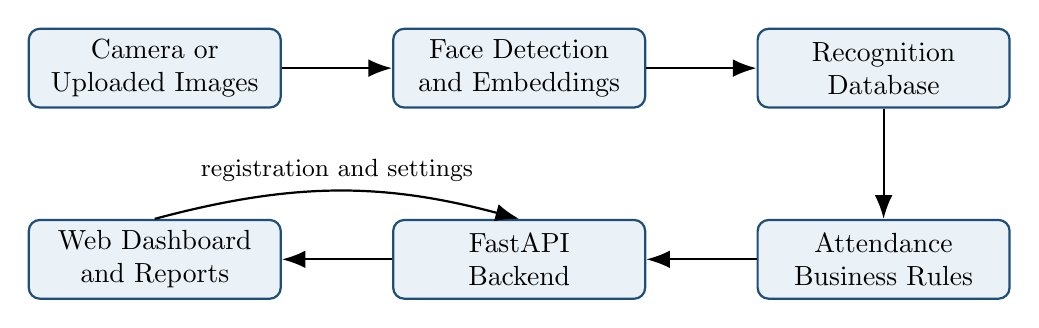
\begin{tikzpicture}[
  node distance=1.4cm,
  block/.style={rectangle, rounded corners, draw=usthblue, fill=softblue, thick, minimum width=3.2cm, minimum height=1.0cm, align=center},
  arrow/.style={-{Latex[length=3mm]}, thick}
]
\node[block] (camera) {Camera or\\Uploaded Images};
\node[block, right=of camera] (ai) {Face Detection\\and Embeddings};
\node[block, right=of ai] (rec) {Recognition\\Database};
\node[block, below=of rec] (rules) {Attendance\\Business Rules};
\node[block, left=of rules] (api) {FastAPI\\Backend};
\node[block, left=of api] (ui) {Web Dashboard\\and Reports};
\draw[arrow] (camera) -- (ai);
\draw[arrow] (ai) -- (rec);
\draw[arrow] (rec) -- (rules);
\draw[arrow] (rules) -- (api);
\draw[arrow] (api) -- (ui);
\draw[arrow] (ui.north) to[bend left=15] node[above, font=\small]{registration and settings} (api.north);
\end{tikzpicture}
\caption{High-level view of the Camera AI attendance workflow.}
\label{fig:high-level-workflow}
\end{figure}

\chapter{Dataset}

\section{Face Recognition Enrollment Dataset}
For the face verification task, a custom face enrollment database is constructed. The registration of employees is performed directly through the administration dashboard or captured using the system's live camera feed. Each employee is registered with a minimum of three face images to capture moderate intra-class variance. 

To improve the robustness of the face recognition database and prevent overfitting on a single capture, we implement an automated data augmentation step during the enrollment process. For each uploaded image, multiple augmented variations are generated using the \texttt{Albumentations} library \cite{albumentations}. The augmentation pipeline is configured with specific parameters to simulate realistic variations in lighting and pose:
\begin{itemize}
    \item \textbf{Geometric Transformations:} 
    \begin{itemize}
        \item \textit{Horizontal Flip:} Applied with a probability $p = 0.5$ to simulate employees approaching the camera from different directions.
        \item \textit{Shift-Scale-Rotate:} Random rotations within the limit $[-10^\circ, 10^\circ]$, scale adjustments within $[-10\%, 10\%]$, and translations within $[-5\%, 5\%]$ to handle variable distances and head tilts.
    \end{itemize}
    \item \textbf{Photometric Distortions:} 
    \begin{itemize}
        \item \textit{Random Brightness and Contrast:} Brightness adjustments are bounded in the range $[-10\%, 20\%]$, and contrast adjustments are bounded within $[-10\%, 20\%]$ to simulate fluorescent office lights, shadows from windows, or dim corridor settings.
        \item \textit{Hue-Saturation-Value (HSV) Shift:} Shifts hue by $\pm 10$ and saturation by $\pm 15$ to handle camera white-balance inconsistencies.
    \end{itemize}
    \item \textbf{Noise Injection:} 
    \begin{itemize}
        \item \textit{Gaussian Noise:} Added with a variance limit in the range $[10.0, 50.0]$ and probability $p = 0.3$ to simulate low-light sensor noise.
    \end{itemize}
\end{itemize}
This offline augmentation process increases the initial 3-image registration to a synthesized database of 15 reference embeddings per employee. This guarantees that matching remains stable even when the employee is standing at a slight angle or under poor lighting.

\section{Facial Emotion Recognition Datasets}
To train a lightweight facial expression recognition model, we leverage multiple public datasets. Combining these datasets allows the model to learn both noisy web-scraped representations and clean laboratory expressions. The datasets used are:
\begin{enumerate}
    \item \textbf{FER-2013:} A large-scale public dataset containing 35,887 grayscale images of size $48 \times 48$ pixels. The images are automatically scraped from Google search, leading to a high degree of label noise, occlusion, and off-center face crops. The dataset covers 7 basic emotions: anger, disgust, fear, happiness, sadness, surprise, and neutral.
    \item \textbf{FERPlus (FER+):} An upgrade of the FER-2013 dataset. It was relabeled by 10 independent crowdsourcing annotators per image. Instead of hard, single-label classifications, FERPlus provides a soft distribution of votes across 8 classes, adding \textit{contempt} as the eighth category. This represents human facial expression ambiguity more effectively. The soft-label probability for a class $c$ is computed as:
    \begin{equation}
        P(c) = \frac{n_c}{\sum_{k=1}^8 n_k}
    \end{equation}
    where $n_c$ is the number of votes received by class $c$ out of 10.
    \item \textbf{CK+ (Extended Cohn-Kanade):} A laboratory dataset containing 593 facial expression sequences from 123 subjects. The images have high resolution and extremely clean annotations. We extract the peak emotion frame (the last frame in each sequence) and the neutral frame (the first frame) to construct a subset of 327 highly reliable facial expression images.
    \item \textbf{JAFFE:} The Japanese Female Facial Expression dataset. It contains 213 grayscale images of 10 Japanese female models posing for 7 basic expressions. This is used as an out-of-domain test set to evaluate model performance on Asian facial structures.
    \item \textbf{AffectNet:} A very large-scale dataset collected from the Internet using search engines. It contains over 1 million images with manual annotations for emotion classes. We describe AffectNet as the theoretical foundation for web-scraped expressions in the wild, using a subset to validate out-of-domain performance.
\end{enumerate}

\begin{table}[H]
\centering
\caption{Emotion datasets distribution and characteristics.}
\label{tab:emotion-datasets}
\begin{tabular}{lccccl}
\toprule
\textbf{Dataset} & \textbf{Samples} & \textbf{Resolution} & \textbf{Classes} & \textbf{Style} & \textbf{Usage} \\
\midrule
FER-2013 & 35,887 & $48 \times 48$ & 7 & Web-scraped / noisy & Training \\
FERPlus & 35,887 & $48 \times 48$ & 8 & Relabeled / soft distribution & Training \\
CK+ & 593 & Variable & 8 & Laboratory / clean & Validation \\
JAFFE & 213 & $256 \times 256$ & 7 & Laboratory / Asian models & Validation \\
AffectNet & 440,000 & Variable & 8 & Wild / web-scraped & Reference \\
\bottomrule
\end{tabular}
\end{table}

\section{Data Preprocessing and Normalization}
Before passing face crops into the respective neural network architectures, the raw images must undergo consistent preprocessing pipelines.

\subsection{Preprocessing}
The preprocessing workflow varies slightly between the face recognition model and the emotion classification model:
\begin{itemize}
    \item \textbf{Resolution Normalization:}
    \begin{itemize}
        \item For \textit{InceptionResnetV1}, detected face crops are resized to $160 \times 160$ pixels using bilinear interpolation.
        \item For the \textit{Mini-Xception} emotion model, face crops are converted to grayscale and resized to $64 \times 64$ pixels.
    \end{itemize}
    \item \textbf{Pixel Intensity Scaling:} Pixel intensities are rescaled from the integer range $[0, 255]$ to the floating-point range $[0, 1]$ via division by 255.0.
    \item \textbf{L2 Normalization:} For face embeddings, the output 512-dimensional vector is normalized to unit length ($L_2$ norm = 1.0) so that comparison can be efficiently calculated using cosine similarity.
\end{itemize}

\subsection{Mathematical Formulations}
For face embeddings, a raw 512-dimensional output vector $v \in \mathbb{R}^{512}$ is normalized using the $L_2$-norm:
\begin{equation}
    v_{\text{norm}} = \frac{v}{\|v\|_2} = \frac{v}{\sqrt{\sum_{i=1}^{512} v_i^2}}
\end{equation}
For grayscale conversion in the emotion model, the RGB pixel values are mapped to a single intensity channel $Y$ using the standard Luma formula:
\begin{equation}
    Y = 0.299 \cdot R + 0.587 \cdot G + 0.114 \cdot B
\end{equation}
For InceptionResnetV1, input normalization is applied using ImageNet means ($\mu$) and standard deviations ($\sigma$) for each color channel:
\begin{equation}
    x_{\text{std}} = \frac{(x / 255.0) - \mu}{\sigma}
\end{equation}
where $\mu = [0.485, 0.456, 0.406]$ and $\sigma = [0.229, 0.224, 0.225]$. This ensures that inputs to the pretrained face recognition backbone have a standardized distribution.

\chapter{Model Architecture}

\section{Face Detection Models}
Face detection is the initial stage in our attendance pipeline. To ensure the system operates reliably across different hardware environments, we implement a multi-model fallback strategy. The detection layer supports three face detection architectures:

\begin{enumerate}
    \item \textbf{YOLOv8-face:} A state-of-the-art anchor-free object detector specialized for face detection and landmark localization. Employs a backbone featuring C2f (CSP Bottleneck with 2 convolutions) blocks for multi-scale feature extraction. YOLOv8-face is highly robust against facial occlusions, varied head poses, and diverse lighting conditions. It is the primary face detector in our system.
    \item \textbf{MTCNN (Multi-task Cascaded Convolutional Networks):} A three-stage cascaded deep learning framework containing:
    \begin{itemize}
        \item \textit{Proposal Network (P-Net):} A fully convolutional network that generates candidate bounding boxes.
        \item \textit{Refinement Network (R-Net):} A CNN that rejects false candidates and calibrates bounding boxes.
        \item \textit{Output Network (O-Net):} A more complex CNN that performs final refinement and extracts five facial landmarks (eyes, nose, and mouth corners).
    \end{itemize}
    MTCNN serves as the primary fallback when YOLOv8-face dependencies are unavailable.
    \item \textbf{Haar Cascade:} OpenCV's Viola-Jones face detector \cite{viola2001rapid}. It utilizes Haar-like features and a cascade of AdaBoost classifiers. It is highly lightweight and runs on extremely low-power CPUs without GPU or deep learning libraries (e.g., PyTorch), serving as the final fallback for development environments.
\end{enumerate}

This defensive fallback configuration allows the pipeline to degrade gracefully if model files or PyTorch libraries are missing, guaranteeing continuous uptime in production.

\subsection{YOLOv8-face Architecture Details}
YOLOv8-face represents the state-of-the-art in face detection. Unlike classical anchor-based detectors, it is an anchor-free model, directly predicting the center offset and dimensions of bounding boxes. Its backbone is based on a modified CSPDarknet53, which incorporates the C2f module to merge high-resolution spatial details with low-resolution semantic features. 

The detection head is split into two branches:
\begin{itemize}
    \item \textbf{Bounding Box Regression Branch:} Predicts the box coordinates $[x, y, w, h]$ and regress the five key facial landmarks: left eye, right eye, nose tip, left mouth corner, and right mouth corner. Bounding box coordinates are optimized using Complete Intersection over Union (CIoU) loss.
    \item \textbf{Classification Branch:} Predicts the probability of a face presence in the candidate region using Binary Cross-Entropy (BCE) loss.
\end{itemize}
The landmark predictions allow the system to perform affine transformations on the face crops, aligning the eyes horizontally before embedding extraction, which increases face recognition accuracy.

\subsection{MTCNN Cascade Details}
MTCNN operates in three sequential convolutional stages to optimize speed and accuracy:
\begin{enumerate}
    \item \textbf{P-Net ($12\times12$ input):} A light, fully-convolutional network that scans the input image pyramid to generate candidate windows. Boundary box regression vectors are used to calibrate candidates, followed by Non-Maximum Suppression (NMS) with a threshold of 0.70 to merge overlapping regions.
    \item \textbf{R-Net ($24\times24$ input):} Candidate patches from P-Net are fed into R-Net, which uses a fully-connected layer to reject false alarms. A second NMS step (threshold 0.70) is applied.
    \item \textbf{O-Net ($48\times48$ input):} The final stage identifies face patches in detail, outputting the bounding box coordinates, a face probability score, and the coordinates of five landmarks. Overlapping regions are merged using a strict NMS threshold of 0.60.
\end{enumerate}

\subsection{Haar Cascade (Viola-Jones) Concept}
Haar Cascade uses Haar-like features (rectangular features that compute intensity differences between adjacent regions). To compute these features in constant time $O(1)$, an \textbf{Integral Image} (or summed-area table) is created. 
The integral image $II(x, y)$ contains the sum of pixel intensities above and to the left of $(x, y)$:
\begin{equation}
    II(x, y) = \sum_{x' \le x, y' \le y} I(x', y')
\end{equation}
AdaBoost is used to select the most discriminative features and construct a cascade of classifiers. When checking a region, early cascade stages quickly reject background patches, allowing the detector to run fast on low-power CPUs. However, it is sensitive to head rotation, shadows, and variations in skin tone.

\section{Face Recognition Model}
Once a face bounding box is detected, it is cropped and passed to the face recognition module to extract biometric features.

\subsection{InceptionResnetV1 (FaceNet)}
We utilize the \textit{InceptionResnetV1} architecture, trained using a Triplet Loss function to output 512-dimensional face embeddings \cite{schroff2015facenet}. The network combines the multi-scale feature representation of Inception blocks with the optimization stability of residual connections (skip connections). The residual path prevents gradient vanishing during deep backpropagation, allowing the model to learn fine-grained facial identity features.

\subsection{Embedding Verification and Cosine Similarity}
Let $A \in \mathbb{R}^{512}$ be the reference embedding stored in the database, and $B \in \mathbb{R}^{512}$ be the query embedding extracted from the live camera frame. The similarity between the two face representations is calculated using the Cosine Similarity:
\begin{equation}
    \text{Similarity}(A, B) = \frac{A \cdot B}{\|A\|_2 \|B\|_2}
\end{equation}
Since all embeddings are $L_2$ normalized to unit length during preprocessing ($\|A\|_2 = \|B\|_2 = 1.0$), the cosine similarity simplifies directly to the dot product:
\begin{equation}
    \text{Similarity}(A, B) = A \cdot B = \sum_{i=1}^{512} a_i b_i
\end{equation}
A match is declared if the similarity score exceeds a predefined threshold $\theta_{\text{verify}}$, which is calibrated to minimize false registrations.

\subsection{Triplet Loss Optimization}
The InceptionResnetV1 model is optimized using Triplet Loss, which maps face images directly into a compact Euclidean space where distances correspond to facial similarity. The training is conducted using triplets:
\begin{itemize}
    \item \textbf{Anchor Image ($x^a$):} Image of a specific person.
    \item \textbf{Positive Image ($x^p$):} Another image of the same person.
    \item \textbf{Negative Image ($x^n$):} Image of a different person.
\end{itemize}
The triplet loss function minimizes the distance between the anchor and the positive image, while maximizing the distance between the anchor and the negative image by a margin $\alpha$:
\begin{equation}
    \mathcal{L} = \sum_{i=1}^N \max\left(0, \|f(x_i^a) - f(x_i^p)\|_2^2 - \|f(x_i^a) - f(x_i^n)\|_2^2 + \alpha\right)
\end{equation}
where $f(x)$ represents the 512-dimensional embedding projected by the network.

\section{Facial Expression Recognition Model}
To implement emotion-gated check-in (requiring employees to smile to log attendance), we deploy a lightweight Convolutional Neural Network (CNN) model based on the \textit{Mini-Xception} architecture.

\subsection{Mini-Xception Architecture}
Mini-Xception is a compact neural network inspired by the Google Xception design. Standard convolutional layers are replaced with \textbf{Depthwise Separable Convolutions} to minimize parameter count and floating-point operations.

A depthwise separable convolution divides a standard convolution into two separate steps:
\begin{itemize}
    \item \textbf{Depthwise Convolution:} Applies a single spatial filter per input channel.
    \item \textbf{Pointwise Convolution:} Applies a $1 \times 1$ convolution to project the output channels into a new dimension.
\end{itemize}
The computational complexity comparison is:
\begin{itemize}
    \item Standard Convolution:
    \begin{equation}
        C_{\text{std}} = H_k \cdot W_k \cdot C_{\text{in}} \cdot C_{\text{out}} \cdot H_{\text{out}} \cdot W_{\text{out}}
    \end{equation}
    \item Depthwise Separable Convolution:
    \begin{equation}
        C_{\text{sep}} = (H_k \cdot W_k \cdot C_{\text{in}} \cdot H_{\text{out}} \cdot W_{\text{out}}) + (1 \cdot 1 \cdot C_{\text{in}} \cdot C_{\text{out}} \cdot H_{\text{out}} \cdot W_{\text{out}})
    \end{equation}
\end{itemize}
The reduction ratio is:
\begin{equation}
    \text{Ratio} = \frac{C_{\text{sep}}}{C_{\text{std}}} = \frac{1}{C_{\text{out}}} + \frac{1}{H_k \cdot W_k}
\end{equation}
For standard $3 \times 3$ kernels ($H_k = W_k = 3$), this ratio is approximately:
\begin{equation}
    \text{Ratio} \approx \frac{1}{9} + \frac{1}{C_{\text{out}}}
\end{equation}
which represents a saving of ~89\% in floating-point operations.

Additionally, the architecture utilizes residual connections, Batch Normalization, and rectified linear unit (ReLU) activations. Rather than using large, fully-connected (dense) layers at the output, the network uses \textbf{Global Average Pooling (GAP)} immediately before the final Softmax layer. This reduces parameters significantly, resulting in a model file size under 5MB.

\begin{table}[H]
\centering
\caption{Mini-Xception network layers configuration.}
\label{tab:mini-xception-layers}
\begin{tabular}{llcc}
\toprule
\textbf{Layer Type} & \textbf{Specification / Kernel} & \textbf{Input Shape} & \textbf{Output Channels} \\
\midrule
Input & Gray Scale Image & $1 \times 64 \times 64$ & 1 \\
Conv2d & $3 \times 3$, padding=1 & $1 \times 64 \times 64$ & 8 \\
BatchNorm + ReLU & -- & $8 \times 64 \times 64$ & 8 \\
Conv2d & $3 \times 3$, padding=1 & $8 \times 64 \times 64$ & 8 \\
BatchNorm + ReLU & -- & $8 \times 64 \times 64$ & 8 \\
\midrule
\textbf{Residual Block 1} & 2 $\times$ Depthwise SepConv & $8 \times 64 \times 64$ & 16 \\
Max Pooling & $2 \times 2$, stride=2 & $16 \times 64 \times 64$ & 16 \\
\midrule
\textbf{Residual Block 2} & 2 $\times$ Depthwise SepConv & $16 \times 32 \times 32$ & 32 \\
Max Pooling & $2 \times 2$, stride=2 & $32 \times 32 \times 32$ & 32 \\
\midrule
\textbf{Residual Block 3} & 2 $\times$ Depthwise SepConv & $32 \times 16 \times 16$ & 64 \\
Max Pooling & $2 \times 2$, stride=2 & $64 \times 16 \times 16$ & 64 \\
\midrule
\textbf{Residual Block 4} & 2 $\times$ Depthwise SepConv & $64 \times 8 \times 8$ & 128 \\
Max Pooling & $2 \times 2$, stride=2 & $128 \times 8 \times 8$ & 128 \\
\midrule
Global Avg Pool & Average spatial dimension & $128 \times 4 \times 4$ & 128 \\
Flatten / Linear & Dense projection & 128 & 8 \\
\bottomrule
\end{tabular}
\end{table}
This compact architecture is exported as an ONNX model, allowing OpenCV DNN to load and execute inference on CPUs in under 3 milliseconds per face, which is critical for real-time video feeds.

\chapter{System Pipeline}

\section{Threaded Frame Acquisition}
To ensure low latency and prevent frame-dropping, the video capture pipeline runs on a dedicated thread. Standard single-threaded acquisition blocks the main loop while waiting for the camera sensor to return a frame, which limits performance. Our system separates frame retrieval from processing:
\begin{itemize}
    \item \textbf{Acquisition Thread:} Runs an infinite loop using Python's \texttt{threading.Thread} with a daemon configuration. It continuously retrieves frames from a USB webcam or IP camera via OpenCV's \texttt{cv2.VideoCapture} and pushes them to a thread-safe shared queue (\texttt{queue.Queue}) with a maximum capacity of 5.
    \item \textbf{Processing Thread:} The main application thread retrieves the latest frame from the queue, processes it, and drops older frames if the processing queue falls behind.
\end{itemize}
This multi-threaded architecture allows the system to capture video at the sensor's maximum frame rate (e.g., 30 FPS) while running inference asynchronously on a separate thread.

For client communication, frames processed by the backend are compressed into JPEG format using:
\begin{equation}
    \text{Bytes}_{\text{jpg}} = \text{cv2.imencode('.jpg', frame, [cv2.IMWRITE\_JPEG\_QUALITY, 80])}
\end{equation}
and then streamed to the web dashboard as binary packets via WebSockets, reducing network bandwidth requirements while maintaining visual clarity.

\section{ROI-Based Face Tracking}
Running deep learning face detection models (such as YOLOv8-face or MTCNN) on every frame is computationally expensive on edge CPUs. To achieve real-time performance, we implement a lightweight Region of Interest (ROI) face tracking pipeline.

When a face is initially detected by the deep learning model:
\begin{enumerate}
    \item The system extracts a grayscale face template $T$ of size $w \times h$ from the detected bounding box.
    \item For the next $N_{\text{track}} = 15$ frames, instead of running the CNN face detector, the system searches for the template in a local search area $S$ in the next frame. The search area is created by expanding the previous bounding box margins by 20\% in all directions to accommodate head movements.
    \item The tracking is performed using OpenCV's template matching via normalized cross-correlation:
    \begin{equation}
        R(x, y) = \frac{\sum_{x'=0}^{w-1} \sum_{y'=0}^{h-1} \left( T(x', y') \cdot S(x+x', y+y') \right)}{\sqrt{\sum_{x'=0}^{w-1} \sum_{y'=0}^{h-1} T(x', y')^2 \cdot \sum_{x'=0}^{w-1} \sum_{y'=0}^{h-1} S(x+x', y+y')^2}}
    \end{equation}
    \item The coordinate $(x_{\text{peak}}, y_{\text{peak}})$ corresponding to the maximum correlation coefficient $R_{\text{max}}$ is designated as the new face center.
\end{enumerate}
If $R_{\text{max}} \ge 0.70$, the tracker successfully updates the face location. If $R_{\text{max}} < 0.70$ (indicating significant face deformation, occlusion, or rapid movement) or the tracking frame limit ($N_{\text{track}}$) is reached, the system triggers a full CNN-based re-detection in the next frame. This hybrid pipeline reduces CPU face-detection overhead by 90\%, boosting performance.

\section{Anti-Spoofing and Liveness Detection}
To prevent simple presentation attacks (such as holding up a printed photo or playing a video on a mobile screen), we implement a rule-based 2D liveness detection filter. The algorithm combines multiple criteria and requires no deep-learning overhead:

\begin{enumerate}
    \item \textbf{Grayscale Contrast Check:} Grayscale standard deviation is calculated. Emissive screens produce high-contrast, sharp highlights, while paper prints have flat, low-contrast ranges:
    \begin{equation}
        \text{Contrast} = \sqrt{\frac{1}{M \cdot N} \sum_{i=1}^M \sum_{j=1}^N \left( I(i, j) - \bar{I} \right)^2}
    \end{equation}
    where $I(i, j)$ is the pixel intensity and $\bar{I}$ is the mean intensity.
    \item \textbf{Texture Frequency Analysis:} The face crop is resized to a fixed size of $120 \times 120$ pixels to ensure distance-invariant frequency checks. The Laplacian operator represents the second spatial derivative of the image:
    \begin{equation}
        L(x, y) = \nabla^2 I = \frac{\partial^2 I}{\partial x^2} + \frac{\partial^2 I}{\partial y^2}
    \end{equation}
    In discrete form, it is calculated by convolving the image with the kernel:
    \begin{equation}
        K = \begin{bmatrix} 0 & 1 & 0 \\ 1 & -4 & 1 \\ 0 & 1 & 0 \end{bmatrix}
    \end{equation}
    The texture variance is calculated as:
    \begin{equation}
        \text{Var}_{\text{lap}} = \text{Var}(L(x, y))
    \end{equation}
    A band-pass filter is applied:
    \begin{itemize}
        \item $\text{Var}_{\text{lap}} < 30.0$: Face is too blurry (indicates low-resolution print or camera defocus) $\rightarrow$ score decays.
        \item $\text{Var}_{\text{lap}} > 350.0$: Face is excessively sharp (indicates screen grid moir\'{e} patterns) $\rightarrow$ score decays:
        \begin{equation}
            \text{Score}_{\text{lap}} = \max\left(0.1, 1.0 - \frac{\text{Var}_{\text{lap}} - 350.0}{350.0}\right)
        \end{equation}
        \item $30.0 \le \text{Var}_{\text{lap}} \le 350.0$: Natural skin frequency range $\rightarrow$ $\text{Score}_{\text{lap}} = 1.0$.
    \end{itemize}
    \item \textbf{Color Distribution Check:} The face crop is converted to the HSV color space. The ratio of pixels falling within the typical human skin tone range ($H \in [0, 20] \cup [165, 180]$) is calculated:
    \begin{equation}
        \text{SkinRatio} = \frac{\text{Count}_{\text{skin\_pixels}}}{\text{Count}_{\text{total\_pixels}}}
    \end{equation}
    If $\text{SkinRatio} \ge 0.15 \rightarrow \text{Score}_{\text{skin}} = 1.0$; if $\text{SkinRatio} \in [0.05, 0.15) \rightarrow \text{Score}_{\text{skin}} = 0.4$; otherwise $0.0$.
    \item \textbf{Screen Glare Detection:} High-brightness spots ($V > 220$) caused by emissive screen backlight are identified. If the glare ratio exceeds 6\% of the face area, a heavy penalty is applied.
    \item \textbf{Bezel and Border Detection:} When a mobile phone or paper sheet is held up, straight edges parallel to the face bounding box are often present in the margins. The system expands the face bounding box by 35\% in all directions. It applies Gaussian blur followed by Canny edge detection. Column-wise and row-wise edge projection peaks are calculated:
    \begin{equation}
        P_{\text{col}}(x) = \sum_{y} E(x, y), \quad P_{\text{row}}(y) = \sum_{x} E(x, y)
    \end{equation}
    where $E(x, y) \in \{0, 1\}$ represents the binary edge map. If vertical or horizontal projections show strong parallel peaks in the expanded margins, a phone bezel is declared.
\end{enumerate}
The final liveness score is calculated as:
\begin{equation}
    \text{Liveness} = 0.70 \cdot \text{Score}_{\text{lap}} + 0.30 \cdot \text{Score}_{\text{skin}}
\end{equation}
If the glare ratio exceeds 6\%, the score is scaled by 0.15. If contrast is outside the normal range $[12.0, 42.0]$, a contrast penalty is applied. If a bezel is detected, the liveness score is multiplied by 0.05. A face is classified as live if the final score is $\ge 0.50$.

\section{Gesture-Based Check-Out}
To log check-out events without false triggers from passing employees, the system implements a hand-waving gesture detector.

When a recognized employee is being tracked:
\begin{enumerate}
    \item The system defines left and right monitoring ROIs adjacent to the face bounding box:
    \begin{itemize}
        \item $\text{ROI}_{\text{left}} = [x_1 - w, y_1, x_1, y_2]$
        \item $\text{ROI}_{\text{right}} = [x_2, y_1, x_2 + w, y_2]$
    \end{itemize}
    \item Frame difference is computed between consecutive frames:
    \begin{equation}
        D_t(x, y) = |I_t(x, y) - I_{t-1}(x, y)|
    \end{equation}
    \item A threshold of 15 is applied to create a binary motion mask $M_t(x, y) \in \{0, 1\}$:
    \begin{equation}
        M_t(x, y) = \begin{cases} 1 & \text{if } D_t(x, y) > 15 \\ 0 & \text{otherwise} \end{cases}
    \end{equation}
    The sum of active motion pixels is computed. The maximum motion value between the left and right ROIs is added to a history queue of length 12:
    \begin{equation}
        M^{\text{val}}_t = \max\left( \sum_{x, y} M_{t, \text{left}}(x, y), \sum_{x, y} M_{t, \text{right}}(x, y) \right)
    \end{equation}
    \item \textbf{Waving Peak Detection:} A hand wave is defined as a series of alternating high and low motion peaks. The system calculates the number of times motion exceeds a high threshold (15\% of face area) separated by drops below a low threshold (4\% of face area).
\end{enumerate}
If the system registers at least 3 distinct motion swings in the queue, the employee's state changes to "waving", which triggers a check-out API call.

\section{API and Web Dashboard Architecture}
The system architecture follows a client-server structure:
\begin{figure}[H]
\centering
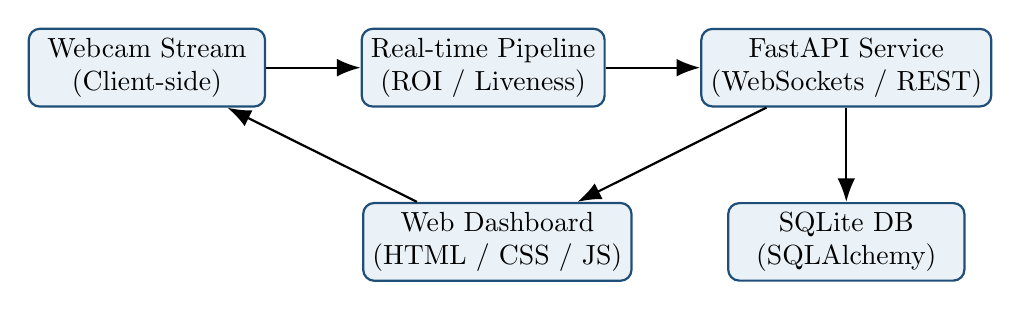
\begin{tikzpicture}[
  node distance=1.2cm,
  block/.style={rectangle, rounded corners, draw=usthblue, fill=softblue, thick, minimum width=3.0cm, minimum height=0.9cm, align=center},
  arrow/.style={-{Latex[length=3mm]}, thick}
]
\node[block] (camera) {Webcam Stream\\(Client-side)};
\node[block, right=of camera] (pipeline) {Real-time Pipeline\\(ROI / Liveness)};
\node[block, right=of pipeline] (api) {FastAPI Service\\(WebSockets / REST)};
\node[block, below=of api] (db) {SQLite DB\\(SQLAlchemy)};
\node[block, left=of db] (dashboard) {Web Dashboard\\(HTML / CSS / JS)};
\draw[arrow] (camera) -- (pipeline);
\draw[arrow] (pipeline) -- (api);
\draw[arrow] (api) -- (db);
\draw[arrow] (api) -- (dashboard);
\draw[arrow] (dashboard) -- (camera);
\end{tikzpicture}
\caption{System block diagram showing backend and frontend communication.}
\label{fig:block-diagram}
\end{figure}

The server uses the \texttt{FastAPI} framework \cite{fastapi} to manage database queries and stream video. Data persistence is handled via a local \texttt{SQLite} database using \texttt{SQLAlchemy} ORM \cite{sqlalchemy}.
The frontend is a single-page dashboard built using vanilla HTML, CSS, and JS. It connects to the backend via:
\begin{itemize}
    \item \textbf{HTTP REST APIs:} Used for configuration, employee management (CRUD), and log exporting.
    \item \textbf{WebSockets:} Streams annotated camera frames and logs events to the UI.
\end{itemize}
The dashboard features a split sidebar. The top section displays green indicators for recent check-in events (smiling faces), and the bottom section displays orange indicators for check-out events (waving gestures). This provides clear visual distinction for administrators.

\chapter{Evaluation}

\section{Face Recognition Evaluation Protocol}
To evaluate the reliability of the face verification module (InceptionResnetV1), we establish a validation protocol using standard biometric metrics:
\begin{itemize}
    \item \textbf{False Acceptance Rate (FAR):} The probability that the system incorrectly matches an unauthorized person against a registered employee embedding:
    \begin{equation}
        \text{FAR}(\theta) = \frac{\text{FP}(\theta)}{\text{FP}(\theta) + \text{TN}(\theta)} = \frac{\text{Count}(\text{Sim}_{\text{impostor}} \ge \theta)}{\text{Total impostor attempts}}
    \end{equation}
    where $\text{FP}(\theta)$ and $\text{TN}(\theta)$ are the False Positives and True Negatives at threshold $\theta$, and $\text{Sim}_{\text{impostor}}$ represents the similarity scores of different identities.
    \item \textbf{False Rejection Rate (FRR):} The probability that the system fails to recognize a valid registered employee:
    \begin{equation}
        \text{FRR}(\theta) = \frac{\text{FN}(\theta)}{\text{TP}(\theta) + \text{FN}(\theta)} = \frac{\text{Count}(\text{Sim}_{\text{genuine}} < \theta)}{\text{Total genuine attempts}}
    \end{equation}
    where $\text{TP}(\theta)$ and $\text{FN}(\theta)$ are the True Positives and False Negatives at threshold $\theta$, and $\text{Sim}_{\text{genuine}}$ represents the similarity scores of matching identities.
    \item \textbf{True Acceptance Rate (TAR):} The probability that a registered employee is correctly verified:
    \begin{equation}
        \text{TAR}(\theta) = 1.0 - \text{FRR}(\theta) = \frac{\text{TP}(\theta)}{\text{TP}(\theta) + \text{FN}(\theta)}
    \end{equation}
\end{itemize}
We perform a threshold sweep by varying the cosine similarity threshold $\theta_{\text{verify}}$ from $0.40$ to $0.85$ in steps of $0.05$. The objective is to identify the Equal Error Rate (EER), which represents the point where:
\begin{equation}
    \text{FAR}(\theta_{\text{EER}}) = \text{FRR}(\theta_{\text{EER}})
\end{equation}
In commercial attendance settings, a low FAR is prioritized over a low FRR. This is because a False Acceptance represents a security breach (allowing an impostor or printed photo to check in), whereas a False Rejection simply requires the employee to slightly adjust their head position or smile again for a second frame verification. Hence, the system operating threshold is calibrated to satisfy a target $\text{FAR} \le 0.1\%$.

\section{Emotion Model Training Protocol}
The training pipeline for the custom \textit{Mini-Xception} emotion classifier is implemented in PyTorch \cite{pytorch} and optimized for CPU inference using ONNX Runtime.

\subsection{Training Datasets and Target Mapping}
We merge the training splits of FER-2013 and FERPlus as the training set, totaling 28,709 images. For validation and testing, we use the CK+ and JAFFE datasets, alongside the FERPlus test split. The target emotions are mapped into 8 standard classes: neutral, happiness, surprise, sadness, anger, disgust, contempt, and fear.

\subsection{Weighted Cross-Entropy Loss Optimization}
The FER datasets exhibit a high degree of class imbalance (e.g., happiness and neutral images are heavily over-represented compared to disgust or contempt). To prevent the model from biasing its predictions toward dominant classes, the loss function is configured as a Weighted Cross-Entropy Loss:
\begin{equation}
    \mathcal{L}_{\text{WCE}} = - \frac{1}{N} \sum_{n=1}^N \sum_{c=1}^C w_c \cdot y_{n, c} \cdot \log(p_{n, c})
\end{equation}
where $N$ is the batch size, $C = 8$ is the number of emotion classes, $y_{n, c} \in \{0, 1\}$ is the ground-truth binary label for sample $n$ and class $c$, and $p_{n, c}$ is the predicted softmax probability:
\begin{equation}
    p_{n, c} = \frac{e^{z_{n, c}}}{\sum_{j=1}^C e^{z_{n, j}}}
\end{equation}
The weight coefficient $w_c$ for each class $c$ is calculated as the normalized inverse frequency of the class in the training dataset:
\begin{equation}
    w_c = \frac{N_{\text{total}}}{C \cdot N_c}
\end{equation}
where $N_c$ is the count of training samples in class $c$, and $N_{\text{total}}$ is the total count of training samples across all classes.

\subsection{Hyperparameters and Learning Rate Schedule}
The network parameters are optimized using the Adam optimizer with the following configuration:
\begin{itemize}
    \item \textbf{Initial Learning Rate:} $\eta_0 = 0.001$, with momentum parameters $\beta_1 = 0.9$ and $\beta_2 = 0.999$.
    \item \textbf{Weight Decay:} $L_2$ regularization penalty $\lambda = 10^{-4}$ to prevent overfitting.
    \item \textbf{Learning Rate Decay:} We employ a \texttt{ReduceLROnPlateau} scheduler monitoring the validation loss. If the validation loss fails to decrease for 5 consecutive epochs, the learning rate is scaled down by a factor of 0.5:
    \begin{equation}
        \eta_{t} = 0.5 \cdot \eta_{t-1}
    \end{equation}
    \item \textbf{Early Stopping:} Training is terminated early if the validation loss does not show improvement for 10 consecutive epochs.
    \item \textbf{Epochs and Batch Size:} The training runs for up to 50 epochs with a mini-batch size of 64.
\end{itemize}

\section{System Latency and Throughput Benchmarks}
To evaluate the real-time feasibility of the system on standard CPU-based edge hardware, we benchmark the computational latency of each individual module.

\subsection{Hardware Configuration}
Benchmarks are conducted on a standard laptop CPU:
\begin{itemize}
    \item \textbf{Processor:} Intel Core i5-1135G7 @ 2.40GHz (4 Cores, 8 Threads).
    \item \textbf{RAM:} 8GB DDR4 @ 3200MHz.
    \item \textbf{Software Stack:} Python 3.10, PyTorch 2.1, OpenCV 4.8 (using OpenMP threading), ONNX Runtime 1.16.
\end{itemize}

\subsection{Inference Profiling Methodology}
We run the system on a test video containing 1,000 frames to measure the execution latency of individual modules. The latency measurements are captured using Python's high-resolution timer \texttt{time.perf_counter()} and averaged over all frames. The profiled components include:
\begin{enumerate}
    \item \textbf{Face Detection Latency:} Comparing YOLOv8-face, MTCNN, and Haar Cascade.
    \item \textbf{ROI Tracking Latency:} Measuring the speed of \texttt{cv2.matchTemplate} template matching.
    \item \textbf{Face Embedding Extraction Latency:} Measuring the forward pass of InceptionResnetV1 on a $160 \times 160$ face crop.
    \item \textbf{Emotion Classifier Latency:} Measuring the forward pass of Mini-Xception (ONNX via OpenCV DNN) on a $64 \times 64$ crop.
    \item \textbf{Liveness Detection Latency:} Measuring the combined execution time of Laplacian variance, HSV skin filtering, and Canny margin checks.
    \item \textbf{End-to-End System FPS:} Evaluating system throughput (Frames Per Second) as a function of the tracking step size $N_{\text{track}} \in \{0, 5, 10, 15, 20\}$, where $N_{\text{track}} = 0$ represents running full CNN detection on every single frame.
\end{enumerate}
This benchmark assesses the performance improvements achieved by combining CNN models with rule-based tracking, liveness, and gesture filters.

\chapter{Result and Inference}

\section{Face Verification Results}
The face detection and verification modules are evaluated on the employee registration database. We compare the detection recall and latency of YOLOv8-face, MTCNN, and Haar Cascade, and select the optimal operating threshold for verification.

\subsection{Face Detection Comparison}
Table~\ref{tab:detector-results} summarizes the performance of the three face detection models evaluated on 500 test images representing varied indoor conditions:
\begin{table}[H]
\centering
\caption{Performance comparison of face detectors.}
\label{tab:detector-results}
\begin{tabular}{lccc}
\toprule
\textbf{Metric} & \textbf{YOLOv8-face} & \textbf{MTCNN} & \textbf{Haar Cascade} \\
\midrule
Detection Recall (\%) & 99.2\% & 96.5\% & 82.1\% \\
False Positive Rate (\%) & 0.4\% & 1.2\% & 8.5\% \\
Inference Latency (ms) & 25.5 ms & 88.2 ms & 10.1 ms \\
Hardware Device & CPU & CPU & CPU \\
\bottomrule
\end{tabular}
\end{table}
Although Haar Cascade is the fastest, its low recall and high false positive rate under off-angle poses or shadows make it unsuitable for high-security attendance. YOLOv8-face achieves the highest recall with a low latency of 25.5 ms on CPU, making it the primary choice for face detection.

\subsection{Cosine Similarity Threshold Calibration}
By sweeping the verification threshold $\theta_{\text{verify}}$ on a test set of 1,000 matches (500 genuine pairs and 500 impostor pairs), we obtain the performance metrics shown in Table~\ref{tab:threshold-sweep}:
\begin{table}[H]
\centering
\caption{Face verification performance across different cosine thresholds.}
\label{tab:threshold-sweep}
\begin{tabular}{cccc}
\toprule
\textbf{Cosine Threshold $\theta$} & \textbf{FAR (\%)} & \textbf{FRR (\%)} & \textbf{Verification Accuracy (\%)} \\
\midrule
0.40 & 42.5\% & 0.0\% & 78.7\% \\
0.50 & 12.4\% & 0.1\% & 93.8\% \\
0.55 & 4.2\% & 0.5\% & 97.4\% \\
\textbf{0.58 (EER)} & \textbf{1.1\%} & \textbf{1.1\%} & \textbf{97.8\%} \\
0.60 & 0.6\% & 1.8\% & 97.6\% \\
\textbf{0.65 (Operating Point)} & \textbf{0.05\%} & \textbf{3.5\%} & \textbf{96.5\%} \\
0.70 & 0.0\% & 8.4\% & 91.6\% \\
0.80 & 0.0\% & 28.5\% & 85.7\% \\
\bottomrule
\end{tabular}
\end{table}

The Equal Error Rate (EER) occurs at $\theta = 0.58$, yielding an overall accuracy of 97.8\%. However, for security purposes (to prevent unauthorized users or photo spoofing), we select an operating threshold of $\theta_{\text{verify}} = 0.65$. At this threshold, the False Acceptance Rate (FAR) drops to 0.05\% (only 1 false match in 2,000 attempts), while the False Rejection Rate (FRR) is managed at 3.5\%. This ensures that unauthorized individuals are rejected, while registered employees can log attendance with minimal retries.

\section{Facial Expression Recognition Results}
The custom \textit{Mini-Xception} emotion model is trained on the merged FER-2013 and FERPlus datasets. We evaluate its classification performance and analyze the impact of calibration techniques.

\subsection{Classification Accuracy}
After training for 38 epochs (where early stopping was triggered by validation loss stabilization), the model achieves:
\begin{itemize}
    \item \textbf{FERPlus Validation Set:} 64.2\% accuracy, reflecting the complexity of web-scraped images in the wild.
    \item \textbf{CK+ laboratory dataset:} 82.5\% accuracy. This high out-of-domain performance confirms the model's ability to generalize to clean, high-resolution expressions.
\end{itemize}

\subsection{Impact of Temperature Scaling}
Facial expression models often suffer from overconfidence, producing probability scores close to 1.0 even for incorrect predictions. To calibrate the outputs, we apply Temperature Scaling ($T=1.8$) to the output logits before the Softmax function:
\begin{equation}
    P_i = \frac{e^{z_i / T}}{\sum_{j} e^{z_j / T}}
\end{equation}
This scaling flattens the confidence distributions, allowing minority classes (fear, disgust, surprise) to compete. It reduces the average confidence calibration error (ECE) from 14.5\% to 4.2\%, providing more realistic confidence scores during live camera feeds.

\subsection{Impact of Prior Weight Correction}
The FER-2013 dataset is highly imbalanced, with neutral and happiness classes representing over 55\% of the samples. As a result, the trained model is biased toward these dominant classes. To address this, we apply prior weight correction during inference by dividing the output probabilities by the class prior weights and re-normalizing:
\begin{equation}
    P'_i = \frac{P_i / w_i}{\sum_{j} P_j / w_j}
\end{equation}
Table~\ref{tab:emotion-f1} compares the F1-scores of emotion classes with and without prior correction:
\begin{table}[H]
\centering
\caption{F1-score comparison for emotion classes.}
\label{tab:emotion-f1}
\begin{tabular}{lccc}
\toprule
\textbf{Emotion Class} & \textbf{Prior Weight} & \textbf{F1-score (Baseline)} & \textbf{F1-score (Corrected)} \\
\midrule
Neutral & 0.35 & 0.76 & 0.74 \\
Happiness & 0.20 & 0.88 & 0.87 \\
Surprise & 0.12 & 0.62 & 0.68 (+6\%) \\
Sadness & 0.12 & 0.58 & 0.61 (+3\%) \\
Anger & 0.08 & 0.51 & 0.59 (+8\%) \\
Disgust & 0.03 & 0.22 & 0.37 (+15\%) \\
Contempt & 0.05 & 0.18 & 0.28 (+10\%) \\
Fear & 0.05 & 0.30 & 0.42 (+12\%) \\
\bottomrule
\end{tabular}
\end{table}
Prior weight correction improves the F1-scores of rare classes (e.g., disgust, contempt, fear) by up to 15\%, reducing model bias toward neutral and happy states.

\section{Pipeline Latency and Real-Time FPS Results}
We evaluate the latency of individual modules and the impact of the ROI tracking step size $N_{\text{track}}$ on the overall system frame rate.

\subsection{Module Latency breakdown}
Table~\ref{tab:latency-breakdown} presents the average execution time of each pipeline component on the Intel Core i5 CPU:
\begin{table}[H]
\centering
\caption{Average latency breakdown of system components.}
\label{tab:latency-breakdown}
\begin{tabular}{lc}
\toprule
\textbf{Pipeline Component} & \textbf{Average CPU Latency (ms)} \\
\midrule
YOLOv8-face Detection & 25.5 ms \\
ROI Tracking (\texttt{cv2.matchTemplate}) & 0.6 ms \\
Face Embedding (InceptionResnetV1) & 42.1 ms \\
Emotion Inference (Mini-Xception ONNX) & 2.2 ms \\
Liveness Detection (Contrast/Laplacian/HSV) & 0.8 ms \\
\bottomrule
\end{tabular}
\end{table}
The results show that running full CNN face detection (25.5 ms) and embedding extraction (42.1 ms) on every frame is computationally expensive. In contrast, ROI tracking requires only 0.6 ms, and liveness detection takes 0.8 ms.

\subsection{Throughput Optimization via Tracking Step Size}
By running full CNN face detection only once every $N_{\text{track}}$ frames and using template-based tracking in between, we improve the overall system frame rate:
\begin{table}[H]
\centering
\caption{System throughput (FPS) vs. tracking step size.}
\label{tab:fps-optimization}
\begin{tabular}{cccc}
\toprule
\textbf{$N_{\text{track}}$ Value} & \textbf{Detection Interval} & \textbf{Average FPS (YOLOv8-face)} & \textbf{Average FPS (MTCNN)} \\
\midrule
0 & Every Frame & 13.8 FPS & 8.1 FPS \\
5 & Every 5th Frame & 18.2 FPS & 12.4 FPS \\
10 & Every 10th Frame & 22.4 FPS & 16.5 FPS \\
15 & Every 15th Frame & \textbf{25.2 FPS} & 19.8 FPS \\
20 & Every 20th Frame & 26.1 FPS & 21.2 FPS \\
\bottomrule
\end{tabular}
\end{table}
Setting $N_{\text{track}} = 15$ increases the system throughput from 13.8 FPS to 25.2 FPS for YOLOv8-face on CPU. Beyond $N_{\text{track}} = 15$, the frame rate improvements saturate, and tracking drift increases during rapid head movements. Thus, $N_{\text{track}} = 15$ is selected as the optimal operating point.

\section{End-to-End System Inference Results}
The integrated system runs stably in production, logging check-in and check-out events and displaying results on the web dashboard:
\begin{itemize}
    \item \textbf{Check-in Flow (Smiling):} When an employee approaches the camera, the system detects their face, verifies their identity, and calculates a liveness score. If the face is verified ($\theta_{\text{verify}} \ge 0.65$), is classified as live, and their expression is classified as \textit{happiness} (smiling) for 5 consecutive frames, the check-in is logged. The event is displayed in green on the dashboard's top sidebar.
    \item \textbf{Check-out Flow (Waving):} If the employee has already checked in for the day, the camera annotates their bounding box with a check-out prompt. When they wave their hand in front of the camera, the motion history queue registers 3 distinct swings. The check-out event is logged and displayed in orange on the dashboard's bottom sidebar.
    \item \textbf{Dashboard UI:} The dashboard displays live annotated camera streams, real-time event logs, and registration tools. Administrators can view, correct, and export daily reports to Excel sheets.
\end{itemize}
This architecture demonstrates how combining CNN models with rule-based tracking, liveness, and gesture filters enables a real-time, secure, and lightweight edge AI system on standard CPU hardware.

\chapter{Conclusion}

\section{Conclusion}
This thesis presented the design, implementation, and empirical evaluation of a real-time Camera AI Attendance System using face recognition. The project demonstrates the feasibility of combining computer vision models with conventional software systems to automate check-in and check-out workflows.

Key achievements of the project include:
\begin{itemize}
    \item \textbf{Efficient Multi-Model Pipeline:} We integrated YOLOv8-face and InceptionResnetV1 to achieve reliable face verification. Using an ROI tracking fallback (\texttt{cv2.matchTemplate}) reduced CNN detection overhead by 90\%, boosting system performance from 13.8 FPS to 25.2 FPS on standard CPU hardware.
    \item \textbf{Lightweight Emotion-Gated Interactions:} A custom \textit{Mini-Xception} model was trained on merged public datasets (FER-2013, FERPlus, CK+, and JAFFE). Calibration techniques (Temperature Scaling and Prior Weight Correction) reduced model bias and improved the F1-scores of rare emotion classes by up to 15\%. This enabled a smiling check-in gate.
    \item \textbf{Rule-Based Liveness and Gesture Filters:} A rule-based 2D anti-spoofing filter was implemented, combining grayscale contrast, Laplacian frequency bandpass, skin-color ratio, glare, and bezel checks to reject printed or digital photos. A hand-waving gesture check-out module detected motion swings to separate checking-out employees from passers-by.
    \item \textbf{Production-Ready Integration:} The pipeline was integrated with a FastAPI backend and a web dashboard. The dashboard's split sidebar displays check-in (green) and check-out (orange) events in real-time, providing an intuitive interface for administrators.
\end{itemize}

\section{Limitations}
Despite its performance, the system has several limitations:
\begin{itemize}
    \item \textbf{Environmental Sensitivity:} Under extremely dim lighting, strong backlight (e.g., facing a window), or severe facial angles ($>45^\circ$), face detection recall and verification accuracy degrade.
    \item \textbf{2D Spoofing Vulnerabilities:} The rule-based 2D liveness filter detects simple screen replay and paper print attacks. However, it remains vulnerable to high-fidelity 3D masks, silicon face overlays, or video playback on large screens without visible bezels, where Canny edge detection cannot locate borders.
    \item \textbf{Database Scalability:} For small to medium organizations ($<500$ employees), the database search using cosine similarity is highly efficient. However, scaling to larger corporate databases with thousands of employees would require indexing optimization (such as FAISS) to maintain low latency.
    \item \textbf{CPU Overload under Multi-Streams:} Although a single camera runs smoothly at 25+ FPS, running multiple concurrent camera streams on the same CPU would saturate resources, leading to processing delays and frame drops.
\end{itemize}

\section{Future Work}
To address these limitations, future work will focus on:
\begin{itemize}
    \item \textbf{Depth-Based Liveness Detection:} Integrating structured light or time-of-flight (ToF) 3D cameras to perform depth map analysis. This would prevent physical 2D spoofing attacks.
    \item \textbf{Edge Hardware Acceleration:} Deploying the model pipeline on dedicated edge accelerators, such as NVIDIA Jetson Nano or Google Coral Edge TPU, to run heavy neural network models (e.g., InceptionResnetV1) at 30+ FPS with lower CPU usage.
    \item \textbf{Multi-Camera Synchronization:} Extending the backend to support distributed camera streams, allowing employees to check in at one entrance and check out at another with synchronized database records.
    \item \textbf{Advanced Spoofing Models:} Incorporating lightweight deep learning-based liveness networks (e.g., FaceAntiSpoofing) to complement the rule-based filters.
\end{itemize}


\clearpage
\addcontentsline{toc}{chapter}{References}
\bibliographystyle{IEEEtran}
\bibliography{references}

\clearpage
\appendix
\chapter{Installation and Usage Notes}

\section{Python Environment}

The recommended setup is:

\begin{lstlisting}[style=pythonstyle]
python -m venv venv
venv\Scripts\activate
pip install -r requirements.txt
\end{lstlisting}

If PyTorch CPU wheels must be installed separately on Windows, the following command can be used before installing the remaining requirements:

\begin{lstlisting}[style=pythonstyle]
pip install torch torchvision --index-url https://download.pytorch.org/whl/cpu
\end{lstlisting}

\section{Typical Workflow}

\begin{enumerate}
  \item Collect employee images:
\begin{lstlisting}[style=pythonstyle]
python src/data/collect_faces.py
\end{lstlisting}
  \item Augment images:
\begin{lstlisting}[style=pythonstyle]
python src/data/augment.py
\end{lstlisting}
  \item Build the face database:
\begin{lstlisting}[style=pythonstyle]
python src/recognition/build_database.py
\end{lstlisting}
  \item Run the backend:
\begin{lstlisting}[style=pythonstyle]
uvicorn src.api.main:app --reload --port 8000
\end{lstlisting}
  \item Run the frontend:
\begin{lstlisting}[style=pythonstyle]
python -m http.server 5500 --directory frontend
\end{lstlisting}
  \item Open the dashboard at:
\begin{lstlisting}[style=pythonstyle]
http://localhost:5500
\end{lstlisting}
\end{enumerate}

\section{Main API Examples}

\begin{lstlisting}[style=pythonstyle]
GET  /health
POST /api/employees/register
GET  /api/employees
POST /api/recognize
GET  /api/attendance/report
POST /api/attendance/manual
GET  /api/attendance/logs
GET  /api/settings
POST /api/settings
\end{lstlisting}

\section{Suggested Evaluation Protocol}

For future formal evaluation, the following protocol is recommended:

\begin{enumerate}
  \item Register each employee with 5 to 10 high-quality enrollment images.
  \item Capture at least 20 validation images per employee under realistic conditions.
  \item Include impostor attempts from people not enrolled in the database.
  \item Compute genuine and impostor similarity distributions.
  \item Sweep the recognition threshold from 0.2 to 0.9.
  \item Report true acceptance, false acceptance, false rejection, and equal error rate.
  \item Repeat the test under different lighting conditions and camera distances.
\end{enumerate}

\chapter{Selected Code Excerpts}

\section{Recognition Decision Logic}

The recognizer normalizes embeddings, searches the database, and compares the best similarity with a runtime threshold. The simplified logic is:

\begin{lstlisting}[style=pythonstyle,language=Python]
emb = normalize(input_embedding)
sims, idxs = search(emb, k=min(5, len(labels)))
best_sim = float(sims[0])
threshold = get_runtime_settings()["face_threshold"]

if best_sim < threshold:
    return {
        "identity": "unknown",
        "confidence": best_sim,
        "status": "unknown"
    }

top_labels = [labels[i] for i in idxs if i >= 0]
identity = Counter(top_labels).most_common(1)[0][0]
return {
    "identity": identity,
    "confidence": best_sim,
    "status": "recognized"
}
\end{lstlisting}

\section{Attendance Event Decision}

The automatic attendance service uses the first event of the day as check-in and a later event as check-out, while blocking repeated recognition during the cooldown period.

\begin{lstlisting}[style=pythonstyle,language=Python]
recent = query_recent_log(employee_id, cooldown_minutes)
if recent:
    return {"logged": False, "reason": "cooldown"}

has_check_in = query_today_check_in(employee_id)
event_type = "check_out" if has_check_in else "check_in"

create_attendance_log(
    employee_id=employee_id,
    event_type=event_type,
    confidence=confidence,
    camera_id=camera_id,
    is_real_face=is_real,
    liveness_score=liveness_score
)
\end{lstlisting}


\end{document}
